% -*-coding: utf-8 -*-

\section{Vliv masky na výsledek filtrace}\label{diskuse masky}

    Nyní provedeme diskusi zvolené masky na dvě hlavní vlastnosti filtru: odolnost vůči kontaminaci a snižování variance gaussovského šumu (vysvětlení pojmů viz sekce~\ref{statisticky motivované}). Porovnávat budeme s klasickým průměrovým filtrem, který nejlépe snižuje varianci šumu, ale nemá žádnou odolnost proti kontaminaci a bude nás zajímat, jak se tyto dvě vlastnosti dají efektivně směnit. Nejprve se podíváme na jednodušší filtry medián a BES. U těch má smysl používat binární (viz teorie \ref{statisticky motivované}) masku se sudou kapacitou, neboť pak musíme medián brát jako průměr dvou prostředních prvků, čímž lépe snížíme varianci šumu. Na obrázku~5.1 uvádíme tradiční masky (bez centrálního voxelu) pořadě o kapacitě 6, 18 a 26.

\begin{figure}[h]\label{obr masky}
  \includegraphics[width = \textwidth]{src/5Vysledky/masky.pdf}
  \caption{Tradiční masky}
\end{figure}

    V tabulce~5.1 uvádíme vypočtené hodnoty pro zmíněné dva filtry. Sloupec \emph{snížení variance šumu} udává, jaká bude variance šumu ve filtrovaném obrázku vůči původní. Pro srovnání uvádíme jak snižuje varianci obyčejný aritmetický průměr nad stejnou maskou.

\begin{table}[h]\label{tab med BES}
    \begin{center}
    \begin{tabular}{lllll}
      \toprule
      \multirow{3}{*}{Filtr$_{\mathrm{\substack{kapacita\\ masky}}}$} & max kontamino- & odolnost    & snížení    & snížení variance \\
                                                    & vaných voxelů   & proti       & variance   & šumu čistým      \\
                                                    & v masce         & kontaminaci & šumu       & průměrováním     \\
      \midrule
      medián$_{\mathrm{6}}$             & 2                 & 33,3 \%       & $1/2$    & $1/6$ \\
      medián$_{\mathrm{18}}$            & 8                 & 44,4 \%       & $1/2$    & $1/18$ \\
      medián$_{\mathrm{26}}$            & 12                & 46,2 \%       & $1/2$    & $1/26$  \\
      medián$_{c}$                      & $\lfloor\frac{c+1}{2}\rfloor-1$& $<$ 50 \%& 1 nebo $1/2$& $1/c$\\
      BES$_{\mathrm{6}}$                & 1                 & 16,7 \%       & $1/4$   & $1/6$ \\
      BES$_{\mathrm{18}}$               & 4                 & 22,2 \%       & $1/4$   & $1/18$ \\
      BES$_{\mathrm{26}}$               & 6                 & 23,1 \%       & $1/4$   & $1/26$ \\
      BES$_{c}$                         & $\lceil\frac{c}{4}\rceil-1$& $<$ 25 \%& $3/8$ nebo $1/4$& $1/c$\\
      \bottomrule
    \end{tabular}
    \caption{Vlastnosti filtrů medián a BES}
    \end{center}
\end{table}

    U obecného mediánu pro liché $c$ nedochází ke snížení variance, pro sudé $c$ je to snížení na 1/2. U obecného BES je pro liché $c$ snížení variance 3/8, neboť počítáme varianci veličiny $(X_1 + 2X_2 + X_3)/4$, kde $X_i, i = 1,2,3 \sim N(\mu,\sigma^2)$. Pro sudé $c$ je 1/4 jasná.

    Z tabulky je vidět, že fitry vykazují velkou odolnost vůči kontaminaci (v praxi se pohybuje na max 10 \%) a varianci nesnižují nikterak valně -- v případě mediánu z lichého počtu prvků dokonce vůbec. Lepšího snížení variance šumu na úkor nižší odolnosti vůči kontaminaci dosáhneme použítím Walshova seznamu -- tedy použitím filtrů H.-L. medián a WBES -- kde se se variance sníží navíc \emph{až} dvakrát. Může to být i méně, neboť $\Lw \subset \WL$ a při výběru prvku z $\Lw$ se žádné průměrování nekoná a variance se tak nesnižuje. Dále je třeba si uvědomit, že kontaminace \kk~prvků v masce vede k poškození
    \beq
    \mathrm{f_{bad}}(k) = \sum_{i=0}^{k-1}(c-i)
    \eeq
    prvků ve Walshově listu -- jeden kontaminovaný prvek díky průměrování poškodí dohromady $c$ prvků, druhý dalších $c-1$ (jeden z průměrů již poškozený je) atd. Nejvíce problematické jsou průměry dvou extrémních kontaminovaných prvků, které mají přesně polovinu maximální intenzity a tudíž se neusadí na okrajích seřazeného seznamu -- označme je $p_{\frac{1}{2}}$. Těch může být nejvýše $\lfloor\frac{k}{2}\rfloor\cdot\lceil\frac{k}{2}\rceil$. Definujme $\mathrm{f_{bad}^{-1}}(n)$ jako
    \beq
    \mathrm{f_{bad}^{-1}}(n) = \max\bigg\{k \in \Nn_0 \;\bigg\vert\; n \geq \sum_{i=0}^{k-1}(c-i)\bigg\}
    \eeq
    Pokud budeme postupovat jako u filtrů medián a BES, tzn. že může být \emph{poškozeno} \textit{n} prvků seřazeného \emph{seznamu} až do prvního vybraného (buď medián, nebo první kvartil), což odpovídá $\mathrm{f_{bad}^{-1}}(n)$ kontaminovaným prvkům v \emph{masce}, zajistíme maximálně to, že při konstatních datech, kontaminovaných v příslušném poměru\footnote{respektive tak, že v masce bude vždy maximálně $\mathrm{f_{bad}^{-1}}(n)$ kontaminovaných voxelů}, dá filtr konstatntní výstup, tzn. nezahrne žádné poškozené prvky. Nebude-li však vstup konstantní, mohou se poškozené prvky (a zejména prvky $p_{\frac{1}{2}}$) rozprostřít celkem libovolně po celém seznamu a nijak je neodstraníme. V takovém případě ale prohlašme, že poškozené prvky jsou hodně blízko nějakých \bq zdravých\eq ~prvků a tedy jejich výběr pro výpočet výsledku filtru příliš nevadí. Pro zamezení tomu, aby se prvky ze skupinky $p_{\frac{1}{2}}$ (která drží pohromadě) příliš promítly do výsledku, můžeme indexy vybíraných prvků (medián a kvartily) posunout tak, aby vzdálenost mezi nimi byla větší, než počet $p_{\frac{1}{2}}$ prvků (například pomoc zavedení kvazi-mediánu). Toto ale také zanedbáme s ohledem na předchozí úmluvu.

    V tabulce~5.2 uvádíme výsledy Hodges-Lehmanova mediánu a WBES. Kvůli mediánu je opět vhodné, aby Walshův seznam měl sudý počet prvků, to nastane pokud $4|c \,\vee\, 4|(c+1)$, protože Walshův seznam má ${c+1 \choose 2} = \frac{c(c+1)}{2}$ prvků. Masky tedy použijeme stejné jako na obrázku~5.1, tentokrát ovšem s centrálním voxelem. Vzhledem k tomu, že Walshův seznam obsahuje prvky vzniklé průměrováním dvou různých prvků $\Lw$ i samotné prvky $\Lw$ a my předem nevíme, které prvky filtr vybere, je snížení rozptylu šumu závislé na konkrétních vstupech a jeho analýza je podstatně složitější. Proto se spokojíme pouze s konstatováním, že v praxi je snížení variance u H.-L. medánu a WBES o něco lepší, než u jejich ekvivalentů nevyužívajících Walshův seznam.

\begin{table}[h]
    \begin{center}
    \begin{tabular}{lllll}
      \toprule
      \multirow{4}{*}{Filtr$_{\mathrm{\substack{kapacita\\ masky}}}$}
                                        &délka   & max konta-  & max konta- & odolnost    \\
                                        &Walshova& minovaných  & minovaných & proti       \\
                                        &seznamu & prvků       & voxelů v   & kontami-    \\
                                        &        & ve WL ($n$) & masce $\mathrm{f_{bad}^{-1}}(n)$ & naci \\
      \midrule
      H.-L. med$_{\mathrm{7}}$          & 28  & 13  & 2                 & 28,6 \%      \\
      H.-L. med$_{\mathrm{19}}$         & 190 & 94  & 5                 & 26,3 \%      \\
      H.-L. med$_{\mathrm{27}}$         & 378 & 188 & 8                 & 29,6 \%      \\
      WBES$_{\mathrm{7}}$               & 28  & 6   & 0 (!)             & 0 \%         \\
      WBES$_{\mathrm{19}}$              & 190 & 47  & 2                 & 10,5 \%      \\
      WBES$_{\mathrm{27}}$              & 378 & 94  & 3                 & 11,1 \%      \\
      \bottomrule
    \end{tabular}
    \caption{Vlastnosti filtrů H-L medián a WBES}
    \end{center}
\end{table}\label{tab WBES}

     Vidíme, že zvláště WBES$_{\mathrm{19,27}}$ se odolností proti kontaminaci blíží do teoretických požadovaných mezí. Zajímavá je situace u WBES$_{\mathrm{7}}$, kde je maska tak malá, že filtr, tak jak je navržen, podle naší úmluvy odolný proti kontaminaci není. To můžeme zlepšit tak, že místo prvního a třetího kvartilu vybereme prvky o jedna blíže ke středu pole -- pokozených pak může být 7, což odpovídá jednomu kontaminovanému v masce a 14,3\% odolnosti.
     \vspace{0.5cm}

     V praxi však měříme kontaminaci pro celý obraz a ne na úrovni jednotlivých voxelů. Může se tedy stát, že při 10\% kontaminaci \emph{celého obrazu} nebude výsledek filtru WBES$_{\mathrm{27}}$ příliš dobrý, protože u mnoha voxelů bude kontaminováno více než 10,5 \% okolních voxelů (kontaminované voxely mohou být libovolně rozmístěny) a výstupní voxel bude poškozený -- což ale odpovídá vlastnostem filtru. V odolnosti proti kontaminaci je tudíž dobré mít oproti teoretickým výsledkům nějakou rezervu. Následují praktické ukázky filtrace, včetně demontrace výsledků morfologických filtrů:
     
     \subsection{Výsledky filtrace -- příklady}
     
     Kompletní výsledky všech filtrů pro všechny dále uvedené šumy jsou k dispozici na přiložením DVD. Pro demonstraci filtrů byla opět pouužita stejná data jako pro měření urychlení: 3D SPECT scan mozku o rozměrech $79 \times 95 \times 69$ voxelů v odstínech šedi (0-255). Pro větší zřetelnost byl z výsledku vybrán vždy jeden reprezentativní horizontální řez (konkrétně 31.).
     
     \vspace{0.5cm}
     
     Rozdíly mezi filtry medián, BES, H.-L. medián a WBES předvedeme na kontaminovaném gaussovském šumu s velkou 10\% kontaminací a $\sigma = 10$ při použití datového typu {\tt usigned char}. Poté předvedeme subjektivně nejlepší výsledky (pouze jeden vítězný filtr) pro šum s kontaminací 5 \% a $\sigma = 15$ (agresivní šum) a šum s kontaminací 3 \% a $\sigma = 5$. Parametry šumů jsou poněkud nadsazené kvůli ilustraci schopností filtrů. U řezů vždy ukážeme výsledek filtrace a rozdíl oproti nepoškozenému originálu, pro lepší viditelnost inverzní a vynásobený pěti. Jako subjektivně vítězný fitr jsme pokaždé vybrali ten, kde rozdíl již neměl výrazný chrakter šumu, ale zároveň ještě nedošlo k přílišnému vyhazení (rozdíl byl stále hodně světlý).

    Byla použita maska s poloměrem 1 a kapacitou 27 (poslední na obrázku 5.1) a pro dosažení lepších výsledků maska s poloměrem 2 a kapacitou 80 (krychle $5\times 5\times 5$ bez hran a středu). Čas výpočtu WBES na CPU se pro větší masku pohyboval okolo 40s, H.-L. mediánu okolo 27s, zrychlení na GPU není známo, protože po uplynutí cca 7s bez odezvy CPU kartu resetuje. Navíc zde by byl algoritmus použitý pro tyto filtry extrémě neefektivní kvůli velikosti Walshova seznamu.

    Pro zašumění originálu byla napsána funkce {\tt AddNoise(...)}. V ní je nejprve rozhoduto zda dotyčný voxel bude kontaminovaný -- pokud ne, je pomocí Box-Mulleorvy\footnote{Umožňuje generovat dvě nezávislá N(0,1) rozdělení z dvou nezávislých U(0,1) rozdělení -- ta se dají získat pomocí fukce {\tt rand()}.} formule nagenerován šum s rozdělením N(0,1), který je posléze přetransformován a přičten k hodnotě voxelu.

    U filtrů je opět v dolním indexu uváděna kapacita masky. Samotný šum bez kontaminace uvádíme jen kvůli porovnání, filtry samozřejmě pracují s kontaminovaným šumem. Nyní výsledky pro jednotlivé šumy v pořadí, jak byly popsány (10\%/10, 5\%/15 a 3\%/5):

    \vfill
    \newpage
    \begin{figure}[htp]
        \center
        \begin{minipage}[c]{0.5\textwidth}
            \center
            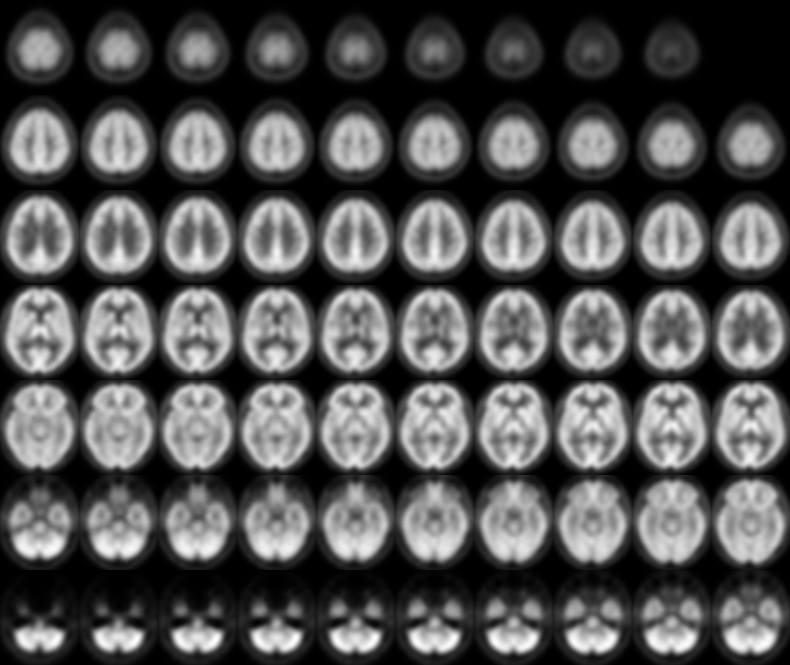
\includegraphics[width = 150pt]{src/8Appendix/final/original.png}
            \caption{Originál}
        \end{minipage}
     \end{figure}
     \begin{figure}[h]
        \begin{minipage}[l]{0.5\textwidth}
            \center
            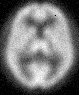
\includegraphics[width = 150pt]{src/8Appendix/final/10-100noise.png}
        \end{minipage}
        \begin{minipage}[r]{0.5\textwidth}
            \center
            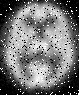
\includegraphics[width = 150pt]{src/8Appendix/final/10-100contaminated.png}
        \end{minipage}
        \\
        \begin{minipage}[l]{0.5\textwidth}
            \caption{Šum, $\sigma = 10$}
        \end{minipage}
        \begin{minipage}[r]{0.5\textwidth}
            \caption{Šum, $\sigma = 10$, kontaminace 10~\%}
        \end{minipage}
    \end{figure}

    \begin{figure}[htp]
        \begin{minipage}[l]{0.5\textwidth}
            \center
            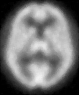
\includegraphics[width = 150pt]{src/8Appendix/final/10-100med.png}
            \caption{Medián$_{27}$}
        \end{minipage}
        \begin{minipage}[r]{0.5\textwidth}
            \center
            
\includegraphics[width = 150pt]{src/8Appendix/final/10-100medD.png}
            \caption{Medián$_{27}$ -- originál}
        \end{minipage}
        \begin{minipage}[l]{0.5\textwidth}
            \center
            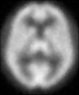
\includegraphics[width = 150pt]{src/8Appendix/final/10-100bes.png}
            \caption{BES$_{27}$}
        \end{minipage}
        \begin{minipage}[r]{0.5\textwidth}
            \center
            
\includegraphics[width = 150pt]{src/8Appendix/final/10-100besD.png}
            \caption{BES$_{27}$ -- originál}
        \end{minipage}
        \begin{minipage}[l]{0.5\textwidth}
            \center
            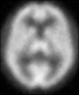
\includegraphics[width = 150pt]{src/8Appendix/final/10-100wmed.png}
            \caption{H.-L. medián$_{27}$}
        \end{minipage}
        \begin{minipage}[r]{0.5\textwidth}
            \center
            
\includegraphics[width = 150pt]{src/8Appendix/final/10-100wmedD.png}
            \caption{H.-L. Medián$_{27}$ -- originál}
        \end{minipage}
    \end{figure}
    \vfill
    \newpage
    ~\vfill~
    \begin{figure}[htp]
        \begin{minipage}[l]{0.5\textwidth}
            \center
            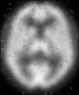
\includegraphics[width = 150pt]{src/8Appendix/final/10-100wbes.png}
            \caption{WBES$_{27}$}
        \end{minipage}
        \begin{minipage}[r]{0.5\textwidth}
            \center
            
\includegraphics[width = 150pt]{src/8Appendix/final/10-100wbesD.png}
            \caption{WBES$_{27}$ -- originál}
        \end{minipage}
    \end{figure}

    \begin{figure}[h]
        \begin{minipage}[l]{0.5\textwidth}
            \center
            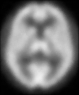
\includegraphics[width = 150pt]{src/8Appendix/final/10-100besL.png}
            \caption{BES$_{80}$ (poloměr 2, vítěz)}
        \end{minipage}
        \begin{minipage}[r]{0.5\textwidth}
            \center
            
\includegraphics[width = 150pt]{src/8Appendix/final/10-100besLD.png}
            \caption{BES$_{80}$ -- originál}
        \end{minipage}
    \end{figure}
    ~\vfill~
    \newpage
    \begin{figure}[Htp] %-----------------------------------------
        \center
        \begin{minipage}[c]{0.5\textwidth}
            \center
            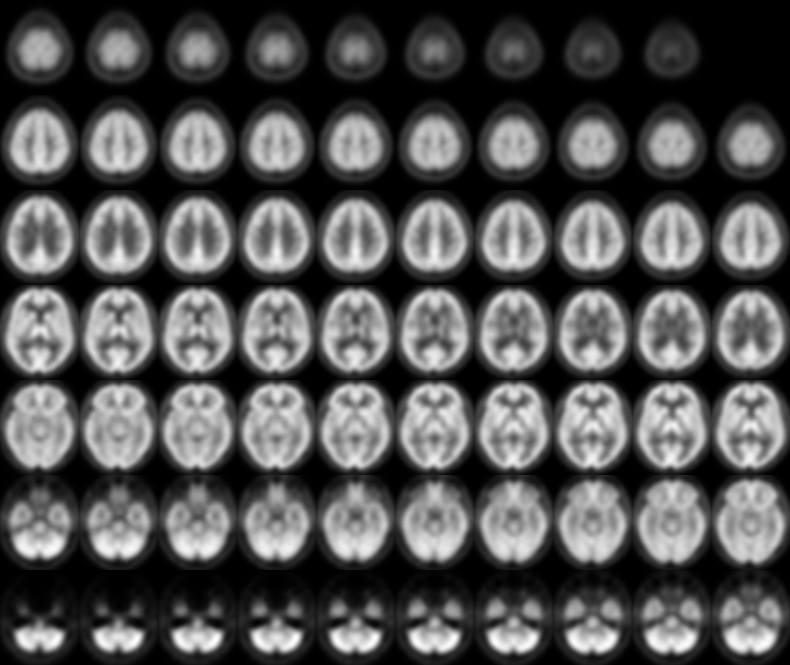
\includegraphics[width = 140pt]{src/8Appendix/final/original.png}
            \caption{Originál}
        \end{minipage}
     \end{figure}\nopagebreak
     \begin{figure}[h!]
        \begin{minipage}[l]{0.5\textwidth}
            \center
            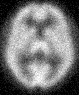
\includegraphics[width = 140pt]{src/8Appendix/final/15-50noise.png}
            %\caption{Zašuměný originál}
        \end{minipage}
        \begin{minipage}[r]{0.5\textwidth}
            \center
            
\includegraphics[width = 140pt]{src/8Appendix/final/15-50contaminated.png}
            %\caption{Zašuměný a kontaminovaný originál}
        \end{minipage}
        \\
        \begin{minipage}[l]{0.5\textwidth}
            \caption{Šum, $\sigma = 15$}
        \end{minipage}
        \begin{minipage}[r]{0.5\textwidth}
            \caption{Šum, $\sigma = 15$, kontaminace 5~\%}
        \end{minipage}
        \begin{minipage}[l]{0.5\textwidth}
            \center
            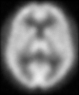
\includegraphics[width = 140pt]{src/8Appendix/final/15-50wbesL.png}
            \caption{WBES$_{80}$ (poloměr 2, vítěz)}
        \end{minipage}
        \begin{minipage}[r]{0.5\textwidth}
            \center
            
\includegraphics[width = 140pt]{src/8Appendix/final/15-50wbesLD.png}
            \caption{WBES$_{80}$ -- originál}
        \end{minipage}
    \end{figure}
    \newpage
    \begin{figure}[Htp]
        \center
        \begin{minipage}[c]{0.5\textwidth}
            \center
            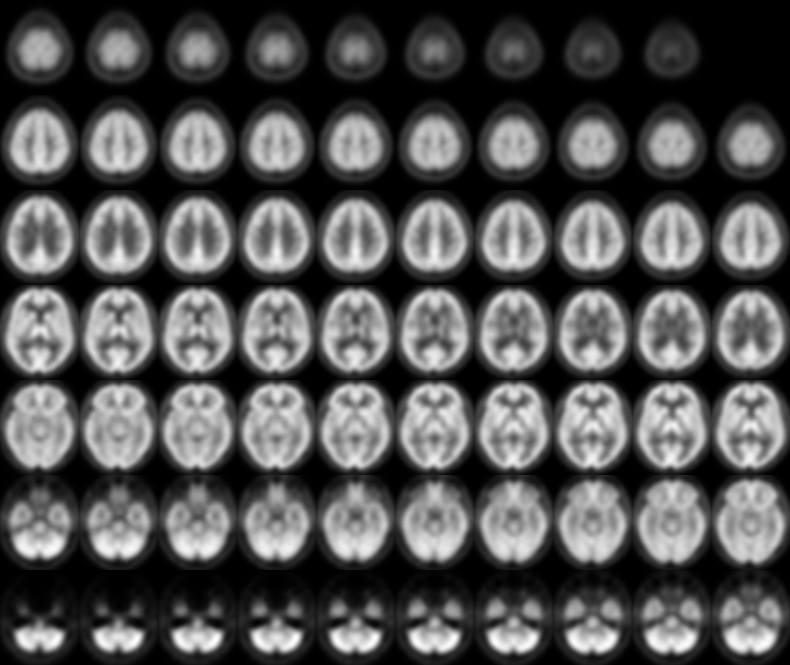
\includegraphics[width = 140pt]{src/8Appendix/final/original.png}
            \caption{Originál}
        \end{minipage}
    \end{figure}
    \begin{figure}[h!]
        \begin{minipage}[l]{0.5\textwidth}
            \center
            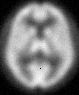
\includegraphics[width = 140pt]{src/8Appendix/final/5-30noise.png}
            %\caption{Zašuměný originál}
        \end{minipage}
        \begin{minipage}[r]{0.5\textwidth}
            \center
            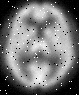
\includegraphics[width = 140pt]{src/8Appendix/final/5-30contaminated.png}
            %\caption{Zašuměný a kontaminovaný originál}
        \end{minipage}
        \\
        \begin{minipage}[l]{0.5\textwidth}
            \caption{Šum, $\sigma = 5$}
        \end{minipage}
        \begin{minipage}[r]{0.5\textwidth}
            \caption{Šum, $\sigma = 5$, kontaminace 3~\%}
        \end{minipage}
        \begin{minipage}[l]{0.5\textwidth}
            \center
            
\includegraphics[width = 140pt]{src/8Appendix/final/5-30bes.png}
            \caption{BES$_{27}$ (vítěz)}
        \end{minipage}
        \begin{minipage}[r]{0.5\textwidth}
            \center
            
\includegraphics[width = 140pt]{src/8Appendix/final/5-30besD.png}
            \caption{BES$_{27}$ -- originál}
        \end{minipage}
    \end{figure}
    \newpage
    
    Vidíme, že u agresivnějších šumů (velká kontaminace, velký rozptyl gaussovského šumu) a nestačí malá maska s poloměrem 1, neboť průměr z tak malého okolí subjektivně nerozpoznáme. Větší maska (poloměr 2) již funguje lépe, ale filtry jsou samozřejmě časově náročnější -- zvláště pak ty na bázi Walshova seznamu. Zde by mohla být alternativou kombinace mediánu (H.-L. mediánu) na malé masce, který odstraní kontaminaci, a nějakého klasického filtru na bázi aritmetického průměru s větší maskou, který se postará o gaussovský šum.
     
     \subsubsection{Ukázky morfologických filtrů}
     
     K vytvoření ukázek filtrů dilatace, eroze a detekce hran byla použita maska s poloměrem 1 a kapacitou 26 (poslední z masek na obrázku 5.1, bez centrálního voxelu). Můžeme vidět, že u detekce hran dochází kvůli nulovým okrajům na stranách obrázku k degeneraci, protože obrázek zasahuje až ke krajům -- zde by bylo vhodnější použít např. okraje s konstantním opakováním.
    \vfill
    \begin{figure}[htp]
        \begin{minipage}[l]{0.5\textwidth}
            \center
            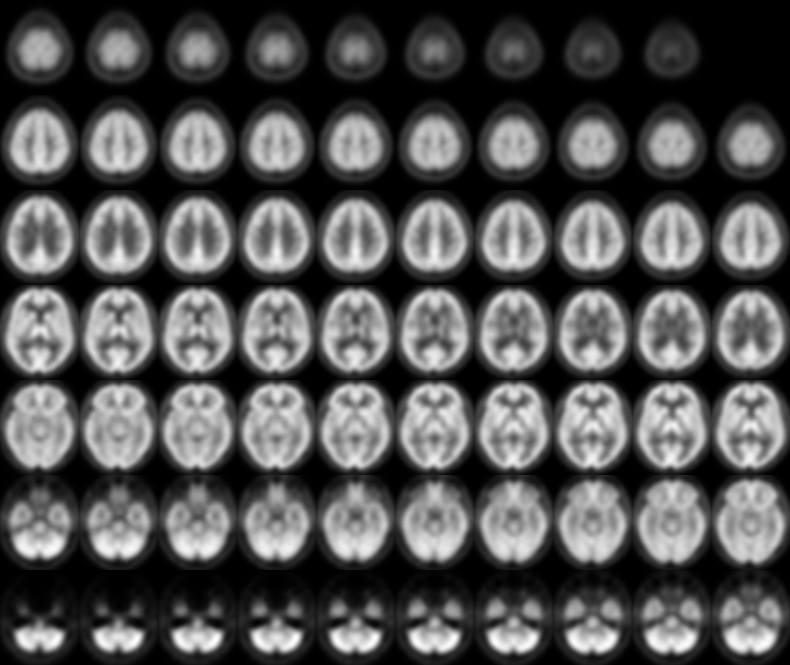
\includegraphics[width = 150pt]{src/8Appendix/final/original.png}
            \caption{Originál}
        \end{minipage}
        \begin{minipage}[r]{0.5\textwidth}
            \center
            
\includegraphics[width = 150pt]{src/8Appendix/final/dilatace.png}
            \caption{Dilatace}
        \end{minipage}
     \end{figure}
     \begin{figure}[h]
        \begin{minipage}[l]{0.5\textwidth}
            \center
            
\includegraphics[width = 150pt]{src/8Appendix/final/eroze.png}
            \caption{Eroze}
        \end{minipage}
        \begin{minipage}[r]{0.5\textwidth}
            \center
            
\includegraphics[width = 150pt]{src/8Appendix/final/hrany.png}
            \caption{Detekce hran}
        \end{minipage}
    \end{figure}
    \vfill
    \newpage
     
\section{Urychlení výpočtů na GPU}

    \subsection{Testovací sestava a data}

    \subsubsection{Data}

        Jako testovací obraz byl použit 3D scan mozku získaný metodou SPECT\footnote{Single Photon Emission Computed Tomography} o rozměrech $79 \times 95 \times 69$ voxelů v odstínech šedi (0-255) uložený ve formátu \Analyze. Pomocí funkce {\tt AddNoise(...)} byl k těmto datům pro demonstraci odstraňování šumu přidám kontaminovaný gaussovský šum s nastavitelnými parametry (viz příloha~\ref{příloha obrázky}).

    \subsubsection{Testovací sestava}

    Filtry jsme testovali na následující sestavě:

    \begin{table}[h]
    \begin{center}
    \begin{tabular}{lcc}
      \toprule
      & CPU & GPU \\
      \midrule
      Název & Intel$^\circledR$ Core$^\mathrm{TM}$ 2 DUO & NVIDIA GeForce 8800 GTX \\
      Výpočetní jednotky & 2 (využita 1) & 128 (4 SM $\times$ 32 CUDA-jader) \\
      Frekvence & 1,86 GHz & 600/1400 MHz (Core/Shader)\\
      Výpočetní schopnost & --- & 1.0 \\
      Cache & 2 MB L2 & --- \\
      RAM/DRAM & 2 GB DDR2 & 768 MB GDDR3 \\
      FSB & 800 MHz & 1800 MHz \\
      \bottomrule
    \end{tabular}
    \caption{Testovací sestava}
    \end{center}
\end{table}

    Program na CPU běžel pouze v jednom vlákně, zde jsme neprováděli žádné paralelní optimalizace.

    \subsection{Výsledky}

    V tabulkách 5.4 a 5.5 uvádíme výsledky pro sedm filtrů popsaných v dřívějších kapitolách. U každého jsme zvolili dvě v praxi používané masky s poloměrem 1. Měření bylo prováděno pomocí rychlého systémového čítače běžícího na frekvenci CPU (1,86 GHz). Každý filtr byl spuštěn 400krát na CPU, 400krát na GPU a to ve 20ti cyklech -- v každém z nich byl spuštěn 20krát bezprostředně za sebou. Při spouštění na GPU byla měřena pouze délka běhu samotného kernelu, režie přesunů dat na GPU nebyla započítána, protože se neprovádí u všech filtrů. Vstupní data byla použita vždy stejná.

    \subsubsection{Morfologické filtry}

\begin{table}[h]\label{výsl 1}
    \hspace{-0.1cm}
    \begin{tabular}{ljkujku}
      \toprule
      Maska $\rightarrow$ & \multicolumn{3}{c}{kapacita masky: 26} & \multicolumn{3}{c}{kapacita masky: 18}\\
      Filtr$_{\frac{vláken}{blok}}$ $\downarrow$ & \multicolumn{1}{c}{CPU (ms)} & \multicolumn{1}{c}{GPU (ms)} & \multicolumn{1}{c}{Urychlení} & \multicolumn{1}{c}{CPU (ms)} & \multicolumn{1}{c}{GPU (ms)} & \multicolumn{1}{c}{Urychlení}\\
      \midrule
      \multicolumn{7}{c}{{\tt unsigned char} (0-255)}  \vspace{0.1cm} \\
      Eroze$_{128}$     & 44,3 & 1,47 & \textbf{30,2} & 32,2 & 1,34 & \textbf{24,0}\\
      Dilatace$_{128}$  & 44,7 & 1,47 & \textbf{30,3} & 32,6 & 1,37 & \textbf{23,8}\\
      Hrany$_{128}$     & 80,7 & 1,56 & \textbf{51,8} & 58,1 & 1,35 & \textbf{43,2}\\
      \midrule
      \multicolumn{7}{c}{{\tt unsigned int} (0-65535)}  \vspace{0.1cm} \\
      Eroze$_{128}$     & 49,8 & 1,61 & \textbf{31,0} & 36,8 & 1,37 & \textbf{26,9}\\
      Dilatace$_{128}$  & 50,0 & 1,62 & \textbf{30,9} & 37,2 & 1,37 & \textbf{27,1}\\
      Hrany$_{128}$     & 78,8 & 1,53 & \textbf{51,4} & 57,3 & 1,32 & \textbf{43,5}\\
      \bottomrule
    \end{tabular}
    \caption{Srovnání morfologických filtrů na CPU a GPU pro různé datové typy}
\end{table}

    Morfologické filtry běžely ve všech variantách se stejnými nastaveními velikosti bloku i počtu bloků. Můžeme vidět několik věcí:
    \begin{itemize}
      \item Rozdíly mezi datovými typy nejsou nijak markantní, ale je zřejmé, že pro typ {\tt unsigned int} zvládá kompilátor o něco lépe optimalizovat a jeho zvýšené paměťové nároky se zde neprojeví.
      \item Při zmenšení masky je zrychlení o něco menší. To je dáno tím, že kernely jsou hodně paměťové vázané a hlavně hodně malé. Tím pádem se při menší masce výrazněji projeví režie a latence.
      \item Hranový detektor (tabulka 5.4, Hrany) vykazuje ve všech případech předpokládané, takřka dvojásobné zrychlení díky lepšímu překrytí paměťových latencí na GPU.
    \end{itemize}

    Další optimalizace těchto kernelů by se mohla zcela jistě ubírat směrem konsolidace práce s pamětí -- nyní vlákno hodnoty přečtené z globální paměti použije jen jednou a v tomto stavu ho nemá smysl optimalizovat. Ideální by bylo zajistit, aby skupina vláken hodnoty sdílela a využít při tom rychlosti sdílené paměti. To by se dalo zařídit například tak, že by blok načetl do sdílené paměti malý krychlový výřez z celého obrazu a filtraci pak prováděl pouze v něm. Každý takto načtený voxel by pak byl použit až tolikrát, kolik je kapacita masky. Otázkou ale zůstává míra efektivity, která by byla hodně závislá na tom, jak široké by byly okraje vůči celému výřezu (ty potřebujeme, ale budou znovupoužity již méněkrát) -- ponechme stranou další nutné režie spojené s kopírováním.

    \subsubsection{Statisticky motivované filtry}

\begin{table}[h]
    \hspace{-0.4cm}
    \begin{tabular}{ljkujku}
      \toprule
      Maska $\rightarrow$ & \multicolumn{3}{c}{kapacita masky: 26} & \multicolumn{3}{c}{kapacita masky: 18}\\
      Filtr$_{\frac{vláken}{blok}}$ $\downarrow$ & \multicolumn{1}{c}{CPU (ms)} & \multicolumn{1}{c}{GPU (ms)} & \multicolumn{1}{c}{Urychlení} & \multicolumn{1}{c}{CPU (ms)} & \multicolumn{1}{c}{GPU (ms)} & \multicolumn{1}{c}{Urychlení}\\
      \midrule
      \multicolumn{7}{c}{{\tt unsigned char} (0-255)}  \vspace{0.1cm}  \\
      Medián$_{192}$        & 320,2 & 9,45      & \textbf{33,9} & 211,3  & 3,62   & \textbf{58,3}\\
      BES$_{192}$           & 377,5 & 10,17     & \textbf{37,1} & 264,0  & 4,98   & \textbf{53,1}\\
      H-L Medián$_{64}$    & 3151,2 & 735,76   & \textbf{4,3}  & 1671,9 & 342,34 & \textbf{4,9} \\
      WBES$_{64}$          & 4704,1 & 1124,46  & \textbf{4,2}  & 2519,9 & 463,81 & \textbf{5,4} \\
      \midrule
      \multicolumn{7}{c}{{\tt unsigned int} (0-65535)}  \vspace{0.1cm} \\
      Medián$_{240}$        & 313,4 & 25,24    & \textbf{12,4} & 206,0  & 5,96   & \textbf{34,6} \\
      BES$_{176}$           & 390,1 & 10,95    & \textbf{35,6} & 274,3  & 6,45   & \textbf{42,5} \\
      H-L Medián$_{64}$    & 3108,3 & 1327,99 & \textbf{2,3}  & 1658,2 & 434,21 & \textbf{3,8}  \\
      WBES$_{64}$          & 4753,3 & 1328,10 & \textbf{3,6}  & 2570,0 & 520,38 & \textbf{4,9}  \\
      \bottomrule
    \end{tabular}
    \caption{Srovnání statistických filtrů na CPU a GPU pro různé datové typy}
\end{table}\label{výsl 2}

    Nyní pobrobněji k statisticky motivovaným filtrům:
    \begin{itemize}
      \item Protože filtry již potřebují větší množství sdílené paměti, je u datového typu {\tt unsigned int} velmi znát jeho čtyřnásobná velikost oproti {\tt unsigned char}. To jsme museli zohlednit ve velikosti bloku (aby se jich na SM vešel optimální počet), což se samozřejmě promítlo do výsledků.
      \item Zrychlení při použítí menší masky se zvětšuje, což je následkem použití \OOO($n^2$) algoritmů, které jsou samozřejmě pro menší pole dat efektivnější, a sofistikovanější (byť optimalizované) algoritmy na CPU zde ztrácí. Zrychlení se nám také u mediánu a BES podařilo udžet na vysoké úrovní díky extenzivnímu využití sdílené paměti.
      \item Algoritmus použitý pro filtry nad Walshovým seznamem je zřejmě příliš triviální a zrychlení je zde dosaženo pouze hrubou výpočetní silou. Optimalizaci by zde mohly pomoci novější karty s větším množstvím paměti a registrů, protože pro CC 1.0 jsou rozměry vstupních dat velmi nepříjemné.
    \end{itemize}

    Zvláštní je zpomalení mediánu při použití většího typu na vetší masce -- je vcelku nezávislé na počtu vláken v bloku (ověřeno experimentem) a při přechodu k menší masce vždy zmizí. Z části jde zřejmě o nešťastnou optimalizaci překladače v kombianci s nevhodnou velikostí masky, z části jde o to, že jsme od začátku optimalizovali algoritmus pro menší datový typ (stejný rozsah jako vstupní data, menší spotřeba paměti), takže nám tyto \bq výstřelky\eq ~zůstaly skryty.

    \vspace{0.5cm}

    Celkově je urychlení na GPU slušné. Zvláště cenné je zrychlení na jednotky ms u \bq menších\eq ~filtrů, které teoreticky umožňuje jejich použití v situacích, kde je třeba výsledek filtrace v reálném čase -- například interaktivní nastavování parametrů filtru. Jakékoliv zrychlení se pak uplatní při konstrukci sítí filtrů, jak bylo zmíněno v sekci~\ref{sítě}.















